
\documentclass[./Thick_TQFTs_and_Quantum_Information.tex]{subfiles}

\begin{document}

\section{Paths for Parallel Transport}

In order to obtain linear maps by parallel transport on manifolds, we need
additional structure on top of connections. These are collections of paths on
manifolds along which we will parallel transport vectors in the fibres of a
bundle with connection. We shall now formalize this apparatus in terms of
categories. We will require a notion of graphs on manifolds whose vertices are
points, possibly repeated, on the manifold and whose edges are paths on the
manifold.

\subsection{Graphs Encoding Monoidal Expression}

We will now define a class of graphs that encode expressions involving tensor
products, point-wise algebra products and composition of linear maps $A \to A$
for some algebra $A$. As a matter of convention, we will take all graphs to mean
directed graphs where we do not allow parallel edges or self-loops. However, we
do allow the underlying undirected graph of any directed graph to be a forest.
Given a graph $G = (V, E)$, we will write $V = V(G)$ and $E(G)$.

\begin{defn}[Elementary Expression Graph]\label{eeg}
Let $G = (V, E)$ be a finite graph satisfying the following properties:
\begin{enumerate}[(i)]

\setlength{\itemsep}{0pt}

\item \label{eeg:part}
$V = V_1 \amalg \dots \amalg V_k$ for some $k \in \N \cup \set{0}$, with each
$V_i$ totally ordered as
$V_i = \set{v_{i, 1}, \dots, v_{i, q_i}}$ for some $q_i \in \N$; note that we
we distinguish between the set $\set{*}$ and the set $\set{v_{i, 1}}$; also, we
keep track of the order of the $V_i$

\item \label{eeg:forward}
for every edge from $u$ to $v$ in $E$, $u \in V_i$ and
$v \in V_{i + 1}$ for some $i \in \set{1, \dots, k - 1}$, when $k \geq 2$

\item \label{eeg:nonredright}
each element in $V_{i + 1}$ has at least one edge from an element in $V_{i}$,
$1 \leq i < k$

\item \label{eeg:nonredleft}
each element in $V_{i}$ has at least one edge to an element in $V_{i + 1}$,
$1 \leq i < k$

\end{enumerate}
Then $G$ is called an elementary expression graph and for any vertex $v \in V$,
we write $p_{G}(v)$ to denote the number $i$ for which $v \in V_i$.
\end{defn}

\begin{rmk}
The total ordering on vertex set parts in condition \eqref{eeg:part} is needed
for defining a ``composition'' or gluing of expression graphs later on.
\end{rmk}

\begin{rmk}
Property \eqref{eeg:forward} above guarantees that $V_1$ has no incoming edges,
$V_k$ has no outgoing edges and there are no edges
``going backwards'' or ``staying within parts'' -- that is, from $V_j$ to $V_i$
for $i \leq j$. It also guarantees that there are no edges ``skipping the next
part'' -- that is, from $V_i$ to $V_j$ for $j > i + 1$.
\end{rmk}

\begin{exm}\label{exm:egraph1}
Consider the graph consisting of nine vertices $1, \dots, 9$ with
$V_1 = \set{1, 2}$, $V_2 = \set{3, 4}$, $V_4 = \set{5, 6, 7}$ and
$V_4 = \set{8, 9}$, along with edges:
\[\begin{array}{ccccc}
  (1, 3) &,& (1, 4) &,& (2, 3),\\
  (3, 5) &,& (3, 6) &,& (4, 7),\\
  (5, 8) &,& (6, 9) &,& (7, 9)
\end{array}\]
It is easy to check that this graph satisfies all conditions in the definition
of an elementary expression graph by visualizing it as follows:
\[\begin{tikzpicture}[baseline=(a).base]
\node[scale=\diagscale] (a) at (0, 0){
\begin{tikzcd}[column sep=huge, row sep=tiny]
                  &                   & 5 \ar[rd] &   \\
1 \ar[r] \ar[rdd] & 3 \ar[ru] \ar[rd] &           & 8 \\
                  &                   & 6 \ar[rd] &   \\
2 \ar[ruu]        & 4 \ar[rd]         &           & 9 \\
                  &                   & 7 \ar[ur] &
\end{tikzcd}
};
\end{tikzpicture}\]

We then observe that we can use this graph to generate an algebraic expression
of the form:
\[
  ((5, 8) \tensor ((6, 9) \cdot (7, 9))) \circ
  ((3, 5) \tensor (3, 6) \tensor (4, 7)) \circ
  (((1, 3) \cdot (2, 3)) \tensor (1, 4))
\]
where the rule is roughly as follows: we infix $(6, 9)$ and $(7, 9)$ with
`$\cdot$' because they share the same target vertex and we call $9$ the target
vertex of $(6, 9) \cdot (7, 9)$; we infix the expressions $(6, 9) \cdot (7, 9)$
and $(5, 8)$ with a `$\tensor$' because they do not share the same target vertex
and we call the expression $5 \tensor 6 \tensor 7$ the source and the expression
$8 \tensor 9$ the target of the expression
$(5, 8) \tensor ((6, 9) \cdot (7, 9))$. For expressions $E_1$ and $E_2$ such
that the target of $E_1$ is the source of $E_2$, we call these expressions
composeable and we form the new expression $E_2 \circ E_1$. This yields the
whole expression above.

One sees readily the edges can be replaced with paths in a manifold $M$ equipped
with an $A$--fibred bundle with connection. These paths can then be replaced
replaced with linear maps $A \to A$ yielding a linear map corresponding to the
expression. We can associate this linear map to $M$ in some notion of TQFT. This
will later motivate us to define an algorithm for obtaining a canonical
expression from an expression graph.
\end{exm}

We observe that we can take disjoint unions of elementary expression graphs but
the result is not an \textit{elementary} expression graph, in general, because
the pieces of the disjoint union do not all have the same number of parts. For
this, we define the following.

\begin{defn}[Expression Graph]
An ordered disjoint union of elementary expression graphs
$G = G_1 \amalg \dots \amalg G_n$ is called an expression graph. We have a part
function for each component expression graph -- that is, $p_{G_i}(u) = j$ if and
only if $u \in G_i$, the vertex set of $G_i$ is $\coprod_{j = 1}^{k_i} V_{i, j}$
and $u \in V_{i, j}$ for some $j$. These collectively give a part function for
$G$ -- $p_G(v) = (i, j) \iff v \in V_{i, j}$
\end{defn}

We now define morphisms of expression graphs.

\begin{defn}[Expression Homomorphism]
A graph homomorphism $h : G \to H$ between expression graphs satisfying
\[
  p_G(u) = p_G(v) \implies p_H(h(u)) = p_H(h(v))
\]
and
\[
  u \leq v \implies h(u) \leq h(v)
\]
\end{defn}

\begin{rmk}
The conditions in the definition above ensures that $h$ restricted to each
elementary expression graph in its domain is also an expression homomorphism
into an elementary expression graph in the codomain.
\end{rmk}

We will now define a notion of gluing for expression graphs. To this end, we
define the ``source'' and ``target'' ends of an expression graph in the obvious
way.

\begin{defn}[Source and Target of an Expression Graph]
Let $G = \coprod_{i = 1}^{n} G_i$ be an expression graph in a manifold $M$ with
$G_i$ having the vertex partition $\coprod_{j = 1}^{k_i} V_{i, j}$. Then, we
define the source of $G$ as the expression graph $S(G)$ with vertex set
$\coprod_{i = 1}^{n} V_{i, 1}$ consisting of a single part and no edges.
The target of $G$ is the expression graph $T(G)$ defined analogously with the
vertex set $\coprod_{i = 1}^{n} V_{i, k_i}$.
\end{defn}

\begin{rmk}
We notice that the total ordering of vertex set parts of each elementary
expression graph in an expression graph along with the ordering of the elementary
expression graphs themselves induces a total ordering of $S(G)$ and $T(G)$,
respectively. At the same time, there are unique inclusion expression
homomorphisms
\[
  S(G) \hto[s_G] G \hot[t_G] T(G)
\]
\end{rmk}

\begin{lem}
Let $G$ and $H$ be expression graphs such that $|S(H)| = |T(G)|$.
We then have a unique expression homomorphism $\psi_{G, H} : T(G) \to S(H)$ which
is monotone on vertex sets. The pushout in $\EG$ of the follosing diagram
exists:
\[
  G \hot[t_G] T(G) \to[\psi_{G, H}] S(H) \hto[s_H] H
\]
\end{lem}
\begin{proof}
We consider the pushout of the diagram in $\Set$ for both the vertex and edge
sets. Then it is easy to see that the resulting vertex and edge sets satisfy the
conditions of the definition of an expression graph -- we are simply identifying
the isomorphic subgraphs $S(H)$ of $H$ and $T(G)$ of $G$ in the disjoint union
$G \amalg H$.
\end{proof}

\begin{defn}[Gluing Expression Graphs]
We define the pushout above to be the gluing $H * G = G \amalg_{S(H)} H$ in
$\EG$. If $G$ and $H$ satisfy the condition $|S(H)| = |T(G)|$ as above, we call
them gluable at $S(H) \cong T(G)$.
\end{defn}

Taking $S(G)$ and $T(G)$ as the identities of $G$ for this gluing operation, it
is straightforward to verify that the associators and unitors for pushouts in
the category of sets are expression homomorphisms. Hence, these associators and
unitors also satisfy associativity and unity coherence axioms to make the
following theorem true. \TODO{Add and appendix entry for the proof of this.}

\subsection{Extracting Expressions}

One immediate way to associate linear maps to a manifold $M$, using the geometry
of the manifold, is to consider an expression graph $G$ with a mapping $\gamma$
of edges to paths on a manifold $M$ equipped with an $A$--fibred bundle
$\pi : E \to M$ along with connection a connection $\nabla$ on $\pi$. In this
case, we can take the linear map obtained by parallel transport of elements of
$A$ along each path in the image of $\gamma$. We can then use $G$ to obtain a
linear map $A^{\amalg |S(G)|} \to A^{\amalg |T(G)|}$, using the same kind of
formula we obtained in example \ref{exm:egraph1}. We are thus motivated to
formalize the notion of an expression associated to an expression graph.

\begin{defn}[Elementary Expression]
Given an elementary expression graph $G$ with vertex set
$\coprod_{i = 1}^{n} V_i$, where each part is ordered as
$V_i = \set{v_{i, 1}, v_{i, 2}, \dots, v_{i, k_i}}$, we define:
\begin{enumerate}[(i)]
\setlength{\itemsep}{0pt}

\item For $j \in \set{1, \dots, k_1}$, the expression associated to $v_{1, j}$
is:
\[
  \Exp{G}_{1, j} := *\footnote{$\varnothing$ is formal symbol.}
\]

\item The expression associated to the vertex set part $V_1$ is:
\[
  \Exp{G}_1 :=
    \overbrace{* \tensor * \tensor \cdots \tensor *}^{k_1 \text{ times}}
\]

\item For
$i \in \set{2, \dots, n}$,
$j \in \set{1, \dots, k_i}$,
let $\set{e_1, e_2, \dots, e_q}$ be the set of incoming edges on $v_{i, j}$,
ordered by the source vertices. Then, the expression associated to $v_{i, j}$
is:
\[
  \Exp{G}_{i, j} := e_1 \cdot e_2 \cdot \cdots \cdot e_q
\]

\item For $i \in \set{2, \dots, n}$, the expression associated to the vertex set
part $V_{i}$ is:
\[
  \Exp{G}_{i} := \Exp{G}_{i, 1} \tensor \Exp{G}_{i, 2} \tensor \cdots
                 \tensor \Exp{G}_{i, k_{i}}
\]

\item The expression associated to $G$ is:
\[
  \Exp{G} := \Exp{G}_n \circ \Exp{G}_{n - 1} \circ \cdots \Exp{G}_{2}
            \circ \Exp{G}_1
\]

\end{enumerate}

Then, $\Exp{G}$ is called the elementary expression of $G$.
\end{defn}

\begin{defn}[Expression]
Given an expression graph $G$ composed of elementary expression graphs
$G_1 \amalg G_2 \amalg \cdots \amalg G_n$, the expression of $G$ is defined as:
\[
  \Exp{G} := \Exp{G_1} \tensor \Exp{G_2} \tensor \cdots \tensor \Exp{G_n}
\]
\end{defn}

\begin{defn}[Expression Composition]
Let $G$ and $H$ expression graphs gluable at $S(H) \cong T(G)$. Then, we have
\[
  \Exp{G} = \Exp{G_1} \tensor \cdots \tensor \Exp{G_n} \text{ and }
  \Exp{G} = \Exp{H_1} \tensor \cdots \tensor \Exp{H_m}
\]
with
\[
  \Exp{G_i} = \Exp{G_i}_{p_i} \circ \cdots \circ \Exp{G_i}_{1} \text{ and }
  \Exp{H_j} = \Exp{H_j}_{q_j} \circ \cdots \circ \Exp{H_j}_{1}
\]
We define:
\[
  \Exp{H} \circ \Exp{G} :=
    \bigotimes_{j = 1}^{m} \Exp{H_j}_{q_j} \circ \cdots \circ \Exp{H_j}_{2}
    \circ \bigotimes_{i = 1}^{n} \Exp{G_i}
\]
\end{defn}

\begin{thm}
Let $h_1, h_2 : G \to H$ be isomorphisms of elementary expression graphs. Then,
$h_1 = h_2$.
\end{thm}
\begin{proof}
Let the vertex parts of $G$ be $V_1 \amalg \cdots \amalg V_n$ and those of $H$
be $V'_1 \amalg \cdots V'_m$. For $n = 1$, we have $V(G) = V_1$ so that there is
$h_1 : V_1 \to V'_j$ is an order-preserving injection for some $j$. However,
$|V(H)| = |V(G)| = |V_1| = |h_1(V_1)|$, so that $V(H) = V'_j = V'_1$ and $h_1$
is an order-preserving bijection $V_1 \to V'_1$. We can argue the same about
$h_2$. Sincer order-preserving bijections between finite sets are unique,
$h_1 = h_2$.

There exists $v \in V_1$ such that $h_1(v) \in V'_j$ for some $j > 1$. There
exists a path $v = v_1v_2 \dots v_n = w$ from $v$ to some $w \in V_n$ such that
$v_i \in V_i$, by the definition of expression graphs. Then,
$h_1(v_1)h_1(v_2) \dots h_1(v_n)$ is a path in $H$ such that
$h_1(v_i) \in V'_{j + i - 1}$. This shows that $m \geq n$. Using $h_1^{-1}$ some
vertex $v' \in V'_1$, we can argue that $n \geq m$ so that $n = m$.
In particular, we must have $j = 1$. We thus have $h_1(V_1) \subset V'_1$. Using
$h_1^{-1}$ in place of $h_1$ in the above argument, we have
$h_1^{-1}(V'_1) \subset V_1 \implies V'_1 \subset h_1(V_1)$, so that
$V_1 = h_1(V'_1)$.

We can repeat this argument with
$h_1|_{G \setminus V_1} : G \setminus V_1 \to H \setminus V'_1$ to show that
$h_1(V_2) = V'_2$ and so on. Then, $h_1|_{V_i} : V_i \to V'_i$ is an order
preserving bijection. We can repeat this argument with $h_2$ so that
$h_1 = h_2$ on all $V_i$. Thus, $h_1 = h_2$.
\end{proof}

\begin{defn}[Equality of Elementary Expressions]
Let $G$ and $H$ be elementary expression graphs. We say that $\Exp{G} = \Exp{H}$
if there exists a (unique) expression isomorphism
$G \stackrel{!}{\longleftrightarrow} H$.
\end{defn}

\begin{defn}[Equality of Expressions]
Let $G$ and $H$ be expression graphs composed of elementary expression graphs
$G_1 \amalg \cdots \amalg G_n$ and $H_1 \amalg \cdots \amalg H_n$ respectively.
Then, we say that $\Exp{G} = \Exp{H}$, if there exists an expression isomorphism
$h : G \longleftrightarrow H$ with $h(G_i) = H_i$ for all $i = 1, \dots, n$.
\end{defn}

\begin{thm}
Let $G$ and $G'$ be expression graphs. Let $H$ be an expression graph gluable
with $G$ at $S(H) \cong T(G)$. Then, we have:
\[
  \Exp{G \amalg G'} = \Exp{G} \tensor \Exp{G'}
\]
and
\[
  \Exp{H * G} = \Exp{H} \circ \Exp{G}
\]
\end{thm}

\begin{defn}[Expression Substitution]
Given an expression graph $G$, we write $\Exp{G}[f]$ to denote the expression
obtained by replacing and edge $(u, v) \in G$ in $\Exp{G}$ with some expression
$f(u, v)$, depending on $(u, v)$.
\end{defn}

\subsection{Geometric Realization}

We wish to use expression graphs to generate linear maps by viewing the edges as
paths in a manifold equipped with an algebra-fibred bundle with connection,
taking their associated parallel transport maps, and combining these maps in a
pattern encoded in the expression graph. To accomplish this, we use the
following simple notion of geometric realization of graphs.

\begin{defn}[Geometric Graph]
A graph in a manifold $M$ or a geometric graph is a graph $G = (V, E)$ equipped
with a function $\gamma : E \to C^0(I, M)$, called a geometric realization of
$G$. We call $M$ the realizing manifold of $G$ under $\gamma$. For an edge from
$u$ to $v$ we write $\gamma_{u, v}$ to denote the path associated to that edge.
\end{defn}

\begin{rmk}
A geometric graph is essentially a collection of paths in a manifold but we
consider one or more copies of each path and ``identify'' their end-points in a
pattern encoded by a graph, even though these paths need not share end-points --
that is, we do not strictly require $\gamma_{u, v}(1) = \gamma_{v, w}(0)$. We
will see that this relaxation is essential to defining our notion of TQFTs. We
will ultimately be interested in expression graphs in manifolds, which will
provide us with a way to associate linear maps to manifolds.
\end{rmk}

\begin{exm}\label{exm:geomegraph}
Consider the graph in example \ref{exm:egraph1}. Then, we consider a mapping of
the edges to paths on a surface as shown below.\footnote{This diagram was
generated using \cite{Mathcha}.} Note that here we have
$\gamma_{u, v}(1) = \gamma_{v, w}(0)$ for most points but not all -- for
instance, $\gamma_{2, 3}$ and $\gamma_{3, 5}$ do not share any end-points.
\begin{figure}[H]
\begin{center}

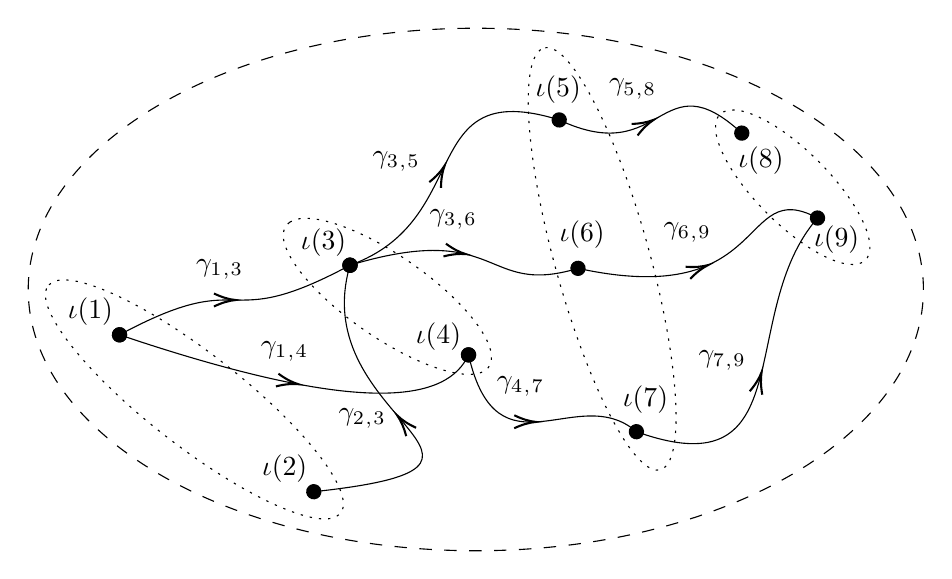
\begin{tikzpicture}[x=0.75pt,y=0.75pt,yscale=-0.95,xscale=0.95]
%uncomment if require: \path (0,281); %set diagram left start at 0, and has height of 281

%Shape: Ellipse [id:dp45216116111361904] 
\draw  [dash pattern={on 4.5pt off 4.5pt}] (6,138.5) .. controls (6,65.32) and (107.63,6) .. (233,6) .. controls (358.37,6) and (460,65.32) .. (460,138.5) .. controls (460,211.68) and (358.37,271) .. (233,271) .. controls (107.63,271) and (6,211.68) .. (6,138.5) -- cycle ;
%Curve Lines [id:da12378300176275903] 
\draw    (52.31,161.49) .. controls (119.1,125.59) and (102.4,162.09) .. (169.19,126.19) ;
\draw [shift={(169.19,126.19)}, rotate = 331.74] [color={rgb, 255:red, 0; green, 0; blue, 0 }  ][fill={rgb, 255:red, 0; green, 0; blue, 0 }  ][line width=0.75]      (0, 0) circle [x radius= 3.35, y radius= 3.35]   ;
\draw [shift={(111.13,143.84)}, rotate = 180.1] [color={rgb, 255:red, 0; green, 0; blue, 0 }  ][line width=0.75]    (10.93,-3.29) .. controls (6.95,-1.4) and (3.31,-0.3) .. (0,0) .. controls (3.31,0.3) and (6.95,1.4) .. (10.93,3.29)   ;
\draw [shift={(52.31,161.49)}, rotate = 331.74] [color={rgb, 255:red, 0; green, 0; blue, 0 }  ][fill={rgb, 255:red, 0; green, 0; blue, 0 }  ][line width=0.75]      (0, 0) circle [x radius= 3.35, y radius= 3.35]   ;
%Curve Lines [id:da3902364739215902] 
\draw    (169.19,126.19) .. controls (233.04,103.33) and (202.45,29.92) .. (275.29,52.51) ;
\draw [shift={(275.29,52.51)}, rotate = 17.23] [color={rgb, 255:red, 0; green, 0; blue, 0 }  ][fill={rgb, 255:red, 0; green, 0; blue, 0 }  ][line width=0.75]      (0, 0) circle [x radius= 3.35, y radius= 3.35]   ;
\draw [shift={(217.18,75.67)}, rotate = 476.11] [color={rgb, 255:red, 0; green, 0; blue, 0 }  ][line width=0.75]    (10.93,-3.29) .. controls (6.95,-1.4) and (3.31,-0.3) .. (0,0) .. controls (3.31,0.3) and (6.95,1.4) .. (10.93,3.29)   ;
\draw [shift={(169.19,126.19)}, rotate = 340.3] [color={rgb, 255:red, 0; green, 0; blue, 0 }  ][fill={rgb, 255:red, 0; green, 0; blue, 0 }  ][line width=0.75]      (0, 0) circle [x radius= 3.35, y radius= 3.35]   ;
%Curve Lines [id:da5125133831866234] 
\draw    (52.31,161.49) .. controls (178.45,204.05) and (218.84,194.46) .. (229.3,171.66) ;
\draw [shift={(229.3,171.66)}, rotate = 294.65] [color={rgb, 255:red, 0; green, 0; blue, 0 }  ][fill={rgb, 255:red, 0; green, 0; blue, 0 }  ][line width=0.75]      (0, 0) circle [x radius= 3.35, y radius= 3.35]   ;
\draw [shift={(142.99,186.54)}, rotate = 191.16] [color={rgb, 255:red, 0; green, 0; blue, 0 }  ][line width=0.75]    (10.93,-3.29) .. controls (6.95,-1.4) and (3.31,-0.3) .. (0,0) .. controls (3.31,0.3) and (6.95,1.4) .. (10.93,3.29)   ;
\draw [shift={(52.31,161.49)}, rotate = 18.65] [color={rgb, 255:red, 0; green, 0; blue, 0 }  ][fill={rgb, 255:red, 0; green, 0; blue, 0 }  ][line width=0.75]      (0, 0) circle [x radius= 3.35, y radius= 3.35]   ;
%Curve Lines [id:da9936282267570157] 
\draw    (150.83,241.06) .. controls (275.76,227.54) and (145.96,205.62) .. (169.19,126.19) ;
\draw [shift={(169.19,126.19)}, rotate = 286.3] [color={rgb, 255:red, 0; green, 0; blue, 0 }  ][fill={rgb, 255:red, 0; green, 0; blue, 0 }  ][line width=0.75]      (0, 0) circle [x radius= 3.35, y radius= 3.35]   ;
\draw [shift={(193.16,202.39)}, rotate = 409.89] [color={rgb, 255:red, 0; green, 0; blue, 0 }  ][line width=0.75]    (10.93,-3.29) .. controls (6.95,-1.4) and (3.31,-0.3) .. (0,0) .. controls (3.31,0.3) and (6.95,1.4) .. (10.93,3.29)   ;
\draw [shift={(150.83,241.06)}, rotate = 353.83] [color={rgb, 255:red, 0; green, 0; blue, 0 }  ][fill={rgb, 255:red, 0; green, 0; blue, 0 }  ][line width=0.75]      (0, 0) circle [x radius= 3.35, y radius= 3.35]   ;
%Curve Lines [id:da37329721640419344] 
\draw    (229.3,171.66) .. controls (243.97,235.64) and (284.76,184.82) .. (314.44,210.62) ;
\draw [shift={(314.44,210.62)}, rotate = 41] [color={rgb, 255:red, 0; green, 0; blue, 0 }  ][fill={rgb, 255:red, 0; green, 0; blue, 0 }  ][line width=0.75]      (0, 0) circle [x radius= 3.35, y radius= 3.35]   ;
\draw [shift={(263.43,205.67)}, rotate = 180.44] [color={rgb, 255:red, 0; green, 0; blue, 0 }  ][line width=0.75]    (10.93,-3.29) .. controls (6.95,-1.4) and (3.31,-0.3) .. (0,0) .. controls (3.31,0.3) and (6.95,1.4) .. (10.93,3.29)   ;
\draw [shift={(229.3,171.66)}, rotate = 77.09] [color={rgb, 255:red, 0; green, 0; blue, 0 }  ][fill={rgb, 255:red, 0; green, 0; blue, 0 }  ][line width=0.75]      (0, 0) circle [x radius= 3.35, y radius= 3.35]   ;
%Curve Lines [id:da6402293447536181] 
\draw    (169.19,126.19) .. controls (246.58,102.99) and (236.29,142.42) .. (284.82,127.77) ;
\draw [shift={(284.82,127.77)}, rotate = 343.19] [color={rgb, 255:red, 0; green, 0; blue, 0 }  ][fill={rgb, 255:red, 0; green, 0; blue, 0 }  ][line width=0.75]      (0, 0) circle [x radius= 3.35, y radius= 3.35]   ;
\draw [shift={(227.95,120.58)}, rotate = 190.98] [color={rgb, 255:red, 0; green, 0; blue, 0 }  ][line width=0.75]    (10.93,-3.29) .. controls (6.95,-1.4) and (3.31,-0.3) .. (0,0) .. controls (3.31,0.3) and (6.95,1.4) .. (10.93,3.29)   ;
%Curve Lines [id:da7275544623824886] 
\draw    (314.44,210.62) .. controls (399.23,240.98) and (364.55,150.12) .. (406.29,102.26) ;
\draw [shift={(406.29,102.26)}, rotate = 311.09] [color={rgb, 255:red, 0; green, 0; blue, 0 }  ][fill={rgb, 255:red, 0; green, 0; blue, 0 }  ][line width=0.75]      (0, 0) circle [x radius= 3.35, y radius= 3.35]   ;
\draw [shift={(377.94,180.41)}, rotate = 465.08] [color={rgb, 255:red, 0; green, 0; blue, 0 }  ][line width=0.75]    (10.93,-3.29) .. controls (6.95,-1.4) and (3.31,-0.3) .. (0,0) .. controls (3.31,0.3) and (6.95,1.4) .. (10.93,3.29)   ;
%Shape: Ellipse [id:dp21247917365246105] 
\draw  [color={rgb, 255:red, 0; green, 0; blue, 0 }  ,draw opacity=1 ][dash pattern={on 0.84pt off 2.51pt}] (16.54,136.11) .. controls (25.63,126.66) and (66.01,145.03) .. (106.72,177.14) .. controls (147.44,209.25) and (173.08,242.94) .. (163.99,252.39) .. controls (154.9,261.85) and (114.52,243.48) .. (73.81,211.37) .. controls (33.09,179.26) and (7.45,145.57) .. (16.54,136.11) -- cycle ;
%Curve Lines [id:da7880732583039812] 
\draw    (275.29,52.51) .. controls (328.72,77.63) and (326.15,20.9) .. (367.89,59.19) ;
\draw [shift={(367.89,59.19)}, rotate = 42.53] [color={rgb, 255:red, 0; green, 0; blue, 0 }  ][fill={rgb, 255:red, 0; green, 0; blue, 0 }  ][line width=0.75]      (0, 0) circle [x radius= 3.35, y radius= 3.35]   ;
\draw [shift={(323.24,52.43)}, rotate = 512.6] [color={rgb, 255:red, 0; green, 0; blue, 0 }  ][line width=0.75]    (10.93,-3.29) .. controls (6.95,-1.4) and (3.31,-0.3) .. (0,0) .. controls (3.31,0.3) and (6.95,1.4) .. (10.93,3.29)   ;
%Curve Lines [id:da726151739669847] 
\draw    (284.82,127.77) .. controls (383.33,149.3) and (366.22,80.72) .. (406.29,102.26) ;
\draw [shift={(350.78,126.12)}, rotate = 518.99] [color={rgb, 255:red, 0; green, 0; blue, 0 }  ][line width=0.75]    (10.93,-3.29) .. controls (6.95,-1.4) and (3.31,-0.3) .. (0,0) .. controls (3.31,0.3) and (6.95,1.4) .. (10.93,3.29)   ;
%Shape: Ellipse [id:dp20693904539608654] 
\draw  [color={rgb, 255:red, 0; green, 0; blue, 0 }  ,draw opacity=1 ][dash pattern={on 0.84pt off 2.51pt}] (138.62,104.37) .. controls (148.74,97.58) and (179.13,108.92) .. (206.48,129.69) .. controls (233.84,150.47) and (247.81,172.81) .. (237.69,179.59) .. controls (227.57,186.38) and (197.19,175.04) .. (169.83,154.27) .. controls (142.47,133.49) and (128.5,111.15) .. (138.62,104.37) -- cycle ;
%Shape: Ellipse [id:dp4442811176180146] 
\draw  [dash pattern={on 0.84pt off 2.51pt}] (268.26,15.88) .. controls (281.5,13.99) and (305.14,60.41) .. (321.05,119.55) .. controls (336.96,178.69) and (339.13,228.17) .. (325.89,230.05) .. controls (312.64,231.94) and (289.01,185.52) .. (273.09,126.38) .. controls (257.18,67.24) and (255.02,17.76) .. (268.26,15.88) -- cycle ;
%Shape: Ellipse [id:dp2537302094398456] 
\draw  [dash pattern={on 0.84pt off 2.51pt}] (358.5,48.46) .. controls (367.96,43.55) and (391.4,56.66) .. (410.84,77.74) .. controls (430.28,98.83) and (438.37,119.9) .. (428.91,124.82) .. controls (419.45,129.73) and (396.01,116.62) .. (376.57,95.54) .. controls (357.13,74.45) and (349.04,53.37) .. (358.5,48.46) -- cycle ;

% Text Node
\draw (50.31,158.09) node [anchor=south east] [inner sep=0.75pt]    {$\iota ( 1)$};
% Text Node
\draw (148.83,237.66) node [anchor=south east] [inner sep=0.75pt]    {$\iota ( 2)$};
% Text Node
\draw (168.57,122.92) node [anchor=south east] [inner sep=0.75pt]    {$\iota ( 3)$};
% Text Node
\draw (226.84,170.66) node [anchor=south east] [inner sep=0.75pt]    {$\iota ( 4)$};
% Text Node
\draw (262.03,45.25) node [anchor=south west] [inner sep=0.75pt]    {$\iota ( 5)$};
% Text Node
\draw (274.13,119.08) node [anchor=south west] [inner sep=0.75pt]    {$\iota ( 6)$};
% Text Node
\draw (306.28,202.6) node [anchor=south west] [inner sep=0.75pt]    {$\iota ( 7)$};
% Text Node
\draw (364.82,65) node [anchor=north west][inner sep=0.75pt]    {$\iota ( 8)$};
% Text Node
\draw (403.23,105) node [anchor=north west][inner sep=0.75pt]    {$\iota ( 9)$};
% Text Node
\draw (89.78,121.75) node [anchor=north west][inner sep=0.75pt]    {$\gamma _{1}{}_{,}{}_{3}$};
% Text Node
\draw (122.67,163.43) node [anchor=north west][inner sep=0.75pt]    {$\gamma _{1}{}_{,}{}_{4}$};
% Text Node
\draw (162.08,197.67) node [anchor=north west][inner sep=0.75pt]    {$\gamma _{2}{}_{,}{}_{3}$};
% Text Node
\draw (179.33,67.29) node [anchor=north west][inner sep=0.75pt]    {$\gamma _{3}{}_{,}{}_{5}$};
% Text Node
\draw (208.3,96.52) node [anchor=north west][inner sep=0.75pt]    {$\gamma _{3}{}_{,}{}_{6}$};
% Text Node
\draw (242.33,181.1) node [anchor=north west][inner sep=0.75pt]    {$\gamma _{4}{}_{,}{}_{7}$};
% Text Node
\draw (299.22,30.41) node [anchor=north west][inner sep=0.75pt]    {$\gamma _{5}{}_{,}{}_{8}$};
% Text Node
\draw (326.9,103.09) node [anchor=north west][inner sep=0.75pt]    {$\gamma _{6}{}_{,}{}_{9}$};
% Text Node
\draw (344.63,168.21) node [anchor=north west][inner sep=0.75pt]    {$\gamma _{7}{}_{,}{}_{9}$};


\end{tikzpicture}


\end{center}
\caption{An elementary transport graph}
\end{figure}
We notice that the same algebraic expression carries over:
\[
  (\gamma_{5, 8} \tensor (\gamma_{6, 9} \cdot \gamma_{7, 9})) \circ
  (\gamma_{3, 5} \tensor \gamma_{3, 6} \tensor \gamma_{4, 7}) \circ
  ((\gamma_{1, 3} \cdot \gamma_{2, 3}) \tensor \gamma_{1, 4})
\]
\end{exm}

\begin{defn}[Transport Graph]
We call a geometric expression graph with an arbitrary vertex $2$--colouring --
that is, we do not require adjacent vertices to have different colours --
a transport graph.
\end{defn}

\begin{defn}[Geometric Homomorphism]
Let $G$ and $H$ be graphs in manifolds $M$ and $N$ with geometric realizations
$\gamma^G$ and $\gamma^H$ respectively, then a homomorphism $h : G \to H$
equipped with a smooth map $f : M \to N$ making the following diagram commute is
called a geometric homomorphism:
\[
\begin{tikzpicture}[baseline=(a).base]
\node[scale=\diagscale] (a) at (0, 0){
\begin{tikzcd}
E(G) \ar[d, "\gamma^G" left] \ar[r, "h" above] &
E(H) \ar[d, "\gamma^H" right] \\
C^0(I, M) \ar[r, "f_*" below] &
C^0(I, N)
\end{tikzcd}
};
\end{tikzpicture}
\]
where $f_*$ is the post-composition map $g \mapsto f \circ g$.
\end{defn}

\begin{defn}[Transport Homomorphism]
A colour-preserving geometric expression homomorphism of transport graphs is
called a transport homomorphism.
\end{defn}

Pasting commutative squares as the one above along the $\gamma$ sides, we
observe that geometric homomorphisms compose associatively. Taking
$h$ and $f$ as the identity maps yields an identity morphism of geometric
graphs. It is also straightforward to verify that disjoint union gives
geometric graphs along with geometric homomorphisms a monoidal structure with
the empty graph in the empty manifold as the monoidal unit.
\TODO{Add an appendix entry for this.}

We wish to eventually formulate transport graphs as a double category. To this
end, we extend the definition to gluing of expression graphs as gluings of
geometric expression graphs as follows.

\begin{lem}
Let $G$ and $H$ be expression graphs in $d$--dimensional cobordisms
$M : X \to Y$ and $N : Y \to Z$ with geometric realizations $\gamma^G$ and
$\gamma^H$ respectively such that $G$ and $H$ are gluable at $S(H) \cong T(G)$.
Then, there exists a geometric realization
\[
  \gamma^H * \gamma^G : E(H * G) \to C^0(I, N * M)
\]
of $H * G$ in $N * M$.
\end{lem}
\begin{proof}
We can define $\gamma^H * \gamma^G$ piecewise away from $S(H) \cong T(G)$. That
is, we define $(\gamma^H * \gamma^G)(e)$ to be
$\gamma^G(e)$ if $e \in E(G) \setminus E(T(G))$ and to be
$\gamma^H(e)$ if $e \in E(H) \setminus E(S(H))$.
If $e \in E(T(G))$, we choose $(\gamma^H * \gamma^G)(e)$ to be $\gamma^G(e)$ and
if $e \in E(S(H))$, we choose $(\gamma^H * \gamma^G)(e)$ to be
$\gamma^G(\psi_{G, H}^{-1}(e))$\footnote{Recall that $\psi_{G, H}$ is the unique
isomorphism $T(G) \to S(H)$.}, so that $\gamma^H * \gamma^G$ agrees on
$S(H) \cong T(G)$.
\end{proof}

\begin{defn}[Gluing Transport Graphs]
For transport graphs $(G, \gamma^G)$ and $(H, \gamma^H)$ with $S(H) \cong T(G)$
with a transport homomorphism, we define their gluing in the obvious way:
\[
  (H, \gamma^H) * (G, \gamma^G) := (H * G, \gamma^H * \gamma^G)
\]
\end{defn}

This is enough structure to develop a simple system for doing algebra using
paths on a manifold. We develop this primitive notion of TQFTs next. \TODO{I am
not sure if it is appropriate call this a notion of TQFTs.}

\subsection{Single Manifold TQFT}

Consider the following data for a simple monoidal double category:
\begin{enmrt}
\li Object category: objects are totally ordered, $2$--coloured, finite sets;
morphisms are order-preserving, colour-preserving (unique) bijections
$V \stackrel{!}{\longleftrightarrow} V'$

\li Morphism category: objects (horizontal $1$--morphisms) are tuples
$(G, \gamma)$, where for a fixed manifold $M$, a fixed bundle $\pi : E \to M$,
and a fixed connection $\nabla$ on $\pi$, $G$ is a transport graph and $\gamma$
is a geometric realization of $G$ in $M$; morphisms are tuples
\[
  (f_0, f_1, h) : (G_1, \gamma^1) \to (G_2, \gamma^2)
\]
where $(f_0, f_1)$ is a morphism of connections $\nabla \to \nabla$ and
$(f_0, h)$ is a transport isomorphism $(G_1, \gamma^1) \to (G_2, \gamma^2)$
\footnote{It is possible that this condition forces $(f_0, f_1) = (\id, \id)$.}

\li Source functor: $S : G \mapsto S(G)$; for a $2$--morphism $(f_0, f_1, h)$,
$S(f_0, f_1, h)$ is the unique order-preserving bijection
$S(\dom h) \to S(\codom h)$

\li Target functor: $T : G \mapsto T(G)$, defined similarly as $S$

\li Unit functor: $U : V \mapsto V$; $U : f \to f$ -- each finite,
totally-ordered set is a transport graph with no edges and order- and colour-
preserving bijections between finite sets are unique transport isomorphisms

\li Horizontal composition:
$(G_2, \gamma^2) * (G_1, \gamma^1) = (G_2 * G_1, \gamma^2 * \gamma^1)$

\li Horizontal associators: inherited from the categories of sets and manifolds

\li Horizontal unitors: inherited like associators

\li Monoidal product: disjoint union

\li Monoidal unit: empty set for object category, empty graph for morphism
category
\end{enmrt}

It is straightforward to verify that the above data does form a monoidal double
category.

\begin{defn}[Double Category of Transport Graphs in a Manifold]
The above data defines the double category of transport graphs in $M$ and we
denote it as $\TG(M)$. We denote the object category as $\TG(M)_0$ and the
morphism category as $\TG(M)_1$.
\end{defn}

We then consider a double functor defined as follows.

\begin{defn}
For a finite, totally-ordered set $V = \set{v_1, \dots, v_n}$ in $\TG(M)_0$, we
set
\[
  F(V) := \bigotimes_{i = 1}^{n} c(v_i)
\]
where $c(v) = A$ if $v$ is blue and $c(v) = \C$ if $v$ is red,
for some algebra $A$.

For every unique order- and colour-preserving bijection $f : V \to V'$ in
$\TG(M)_0$, we set $F(f) := \id_{F(V)} = \id_{F(V')}$.

For a transport graph $(G, \gamma)$ in $M$ -- an object in $\TG(M)_1$ -- and an
edge $(u, v) \in G$, we denote $\nabla^{\gamma_{u, v}}$ to be the parallel
transport map $A \to A$ obtained from $\gamma_{u, v}$. We then define:
\[
  F\br{\nabla^{\gamma_{u, v}}} := \begin{cases}
    \nabla^{\gamma_{u, v}}
      & u \text{ is blue and } v \text{ is blue} \\
    \text{ev}_{a}\br{\nabla^{\gamma_{u, v}}}
      & u \text{ is red and } v \text{ is blue} \\
    \text{trace}\br{\text{ev}_{a}\br{\nabla^{\gamma_{u, v}}}}
      & u \text{ is red and } v \text{ is red} \\
    \text{trace} \circ \nabla^{\gamma_{u, v}}
      & u \text{ is red and } v \text{ is red}
  \end{cases}
\]
We then obtain a linear map:
\[
  F(G, \gamma) := \Exp{G}[F\br{\nabla^{\gamma_{u, v}}}]
    : F(S(G)) \to F(T(G))
\]
For a $2$--morphism
$(f_0, f_1, h) : (G_1, \gamma_1) \to (G_2, \gamma_2)$ in $\TG(M)_1$, we consider
the path $(r_t, s_t)$ in the isomorphism group of the bundle $\pi$ such that
$(r_0, s_0) = (\id_M, \id_E)$ and $(r_1, s_1) = (f_0, f_1)$. We then have a
smoothly varying family of functions $s_t\gamma : E(G) \to C^0(I, M)$
where $(s_t\gamma)_{u, v} = s_t \circ \gamma_{u, v}$. This yields a smoothly
varying family of linear maps, which we write as:
\[
  F(f_0, f_1, h) := \Exp{G}[s_t\gamma]
    : F(S(G)) \to F(T(G)), t \in [0, 1]
\]
\end{defn}

\TODO{Verify that this data does indeed form a monoidal double functor}

\TODO{Define the codomain double category}

\section{TQFTs from Parallel Transport}

We then observe that if we take the gluing
operation in $\EG_{\CCob_{d}}$ to be given by gluings $\EG$ and $\CCob_{d}$
separately along with the gluing of geometric realizations as above, the gluing
is coherently associative and unital up to geometric expression isomorphisms.
The associators of $\EG$ and $\CCob_{d}$ can be verified to yield geometric
expression isomorphisms. For a boundary manifold $X$, the gluing unit of $X$ is
the cylinder $X \times I$ equipped with the single part expression graph with
the same number of vertices as the components of $X$. This yields a double
category of geometric expression graphs but we need the following definition
first.

\begin{defn}[{\color{blue!55!black} What's a good name?}]
Consdier $\CCob_{d + 1}$. Let $\CCob_{d + 1}^0$ be its object category
consisting of the boundary manifolds. We then have a functor
$\text{Comp} : \CCob_{d + 1}^0 \to \N$, where $\N$ viewed as a discrete
category, given by sending each manifold in $D_0$ to the number of components it
has. Similarly, we can take functor $|S(-)| : \EG_1 \to \N$ sending each
single-part graph to the number of its vertices. The pullback
$\EG \prescript{}{|S(-)|}{\times}_{\text{Comp}} \CCob_{d + 1}^0$ is the category
whose objects are pairs $(G, X)$ with $G \in \EG_1$ and $X \in \CCob_{d + 1}^0$
such that $X$ has the same number of components as the number of vertices in
$G$, and whose morphisms are pairs $(h, f)$ where $h$ is the unique expression
homomorphism and $f$ is a diffeomorphism. We denote this category $\EG_{1, d}$.
\end{defn}

We then have the following theorem. \TODO{Add an appendix entry for the proof.}

\begin{thm}
The following data form a monoidal double category:
\begin{enumerate}[(i)]
\setlength{\itemsep}{0pt}
\item Object Category: $\EG_{1, d}$
\item Morphism Category: $\EG_{\CCob_{d + 1}}^{\text{iso}}$
\item Source Functors, $S$: the expression graph $G$ with
geometric realization $\gamma$ in a cobordism $M : X \to Y$ is sent to the pair
$(S(G), X)$; an expression isomorphism
$(h, f) : (G, M, \gamma^G) \to (H, N, \gamma^H)$
is sent to $(h|_{S(G)}, f|_{X})$
\item Target Functor, $T$: defined similarly
\item Unit Functor, $U$: the pair $(X, G)$ is mapped to $X \times I, G$
\item Horizontal Composition Associators: inherited from the double category
$\CCob_{d + 1}$ of cobordisms and that of expression graphs $\DEG$
\item Horizontal Composition Unitors: inherited just like associators
\item Monoidal Product: disjoint union
\item Monoidal Unit: empty manifold equipped with empty graph
\end{enumerate}
\end{thm}

\begin{defn}[Double Category of Geometric Expression Graphs]
We call the double category of the above theorem the double category of
geometric expression graphs and denote it $\DEG_{\CCob_{d + 1}}$.
\end{defn}

We are now in a position to describe our desired TQFTs. In particular, we will
combine our notion of geometric expression graphs with connections to obtain
linear maps from arbitrary manifolds. We will see that there are multiple ways
that this idea can be formalized.

\end{document}

